\paragraph{Analysis 1}\hfill
\\
\phantom{ } After we connected the circuit in Graph 4.1.1 in the lab instruction, we detected a waveform on our oscilloscope. To calculate its time constant accurately, we need as many data as possible. According to the instruction, we recorded 10 points separately for the original circuit, two-stage and three-stage. When we were selecting our testing points, we tried to pick more where the voltage rose(or fell) more rapidly with time. Also, we noticed that the measurements were not stable on the oscilloscope if its value was too small, so we paused the screen on random to record a relatively accurate number.\\
\phantom{ } When we were measuring the voltages and their according time, we used the Cursor whose type was time and took Channel 2 as its source. We settle one of the cursor at start point of a rising or falling action, and moved the other cursor slightly. We also scaled the width of the waveform to get a more accurate move.\\
\phantom{ } Our recordings for the original circuit are shown in the table below.
\paragraph{Experimental Results}
\begin{table}[htbp]\centering
	\renewcommand\arraystretch{1.5}
	\begin{tabular}{lcl}
		\toprule
		No		&Voltage(V)	&time(ms)	\\
		\midrule
		1		&0.512		&16.0		\\
	
		2		&0.880		&32.0		\\
	
		3		&1.20		&44.0		\\
	
		4		&1.52		&60.0		\\
	
		5		&1.92		&80.0		\\
	
		6		&2.28		&100		\\
	
		7		&2.56		&116		\\
	
		8		&2.60		&124		\\
		
		9		&3.68		&216		\\
		
		10		&4.61		&364		\\
		\bottomrule
	\end{tabular}\\
\end{table}
\phantom{ } Then we apply the data in Excel, we get a plot\ref{fig:2.1}:\\
\begin{figure}[htbp]
	\centering %¾ÓÖÐ
	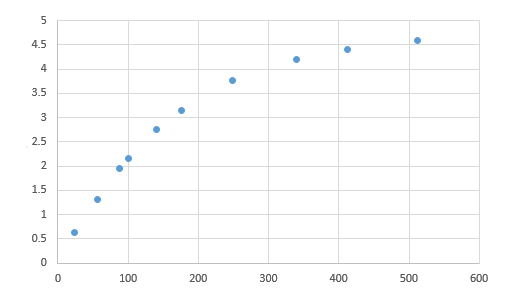
\includegraphics[width=\linewidth]{images/2_1.PNG} %¿í¶È£¬ÎļþµØÖ·
	\caption{plot V-t} %±êÌâ
	\label{fig:2.1} %±ê¼Ç£¨ÒýÓÃʱÓã©
\end{figure}\\
\phantom{ } As the instruction suggested, we made the x-axis(time) into logarithmic and plot again\ref{fig:2.2} :\\
\begin{figure}[htbp]
	\centering %¾ÓÖÐ
	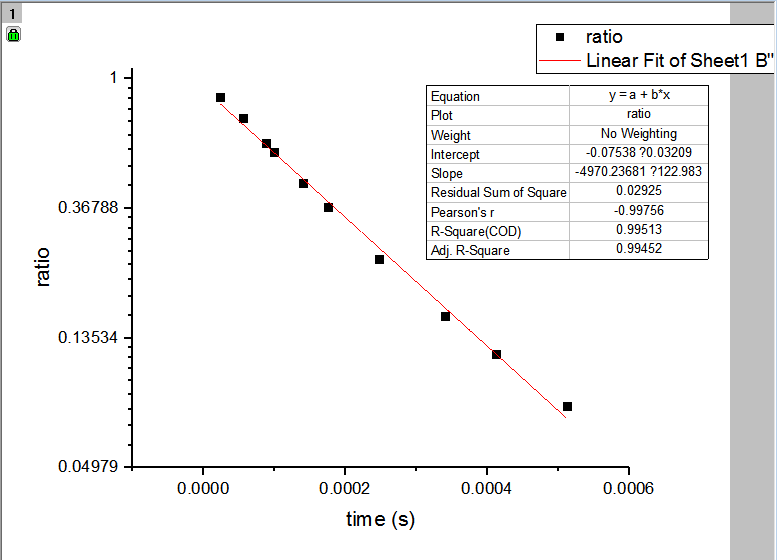
\includegraphics[width=\linewidth]{images/2_2.PNG} %¿í¶È£¬ÎļþµØÖ·
	\caption{plot V-ln(t)} %±êÌâ
	\label{fig:2.2} %±ê¼Ç£¨ÒýÓÃʱÓã©
\end{figure}
\phantom{ } Then we fit a linear line to this plot, and we get a slope of 1.35.
we get its inverse 0.74, which has an 
%\begin{table}[h]\centering
%	\begin{tabular}{}
%		\hline
%		number	&Voltage(V)	&time(ms)	\\
%		\hline
%				&			&			\\
%		\hline
%				&			&			\\
%		\hline
%				&			&			\\
%		\hline
%				&			&			\\
%		\hline
%				&			&			\\
%		\hline
%				&			&			\\
%		\hline
%				&			&			\\
%		\hline
%				&			&			\\
%		\hline
%				&			&			\\
%		\hline
%				&			&			\\
%		\hline
%				&			&			\\
%		\hline
%				&			&			\\
%	\end{tabular}
%\end{table}
	

